\documentclass{standalone}

\usepackage{tikz}
\usepackage{verbatim}

\begin{document}

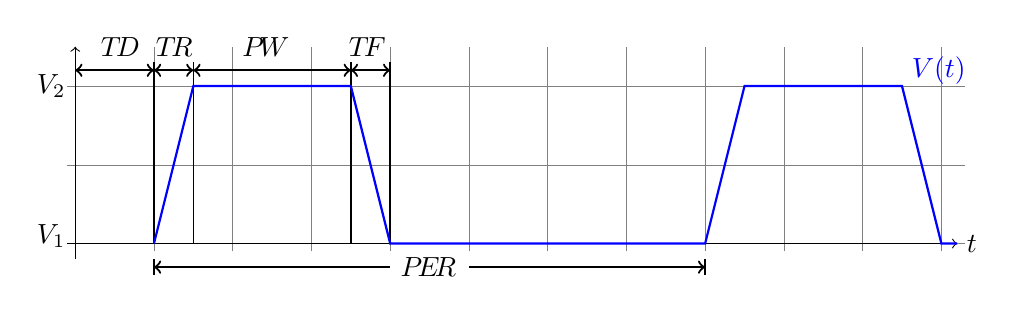
\begin{tikzpicture}[domain=0:11]
    \draw[very thin,color=gray] (-0.1,-0.1) grid (11.3,2.5);
    
    \draw[->] (-0.1,0) -- (11.2,0) node[right] {$t$};
    \draw[->] (0,-.2) -- (0,2.5) node[above] {};
    
    \draw[] (.2,2.5) node[right] {$T\!D$};
    \draw[thick, <->] (0,2.2) -- (1,2.2) node[] {};
    \draw[semithick, -] (1,0) -- (1,2.3) node[] {};

    \draw[] (0.9,2.5) node[right] {$T\!R$};
    \draw[thick, <->] (1,2.2) -- (1.5,2.2) node[] {};
    \draw[semithick, -] (1.5,0) -- (1.5,2.3) node[] {};

    \draw[thick, <->] (1.5,2.2) -- (3.5,2.2) node[] {};
    \draw[] (2.,2.5) node[right] {$P\!W$};
    \draw[semithick, -] (3.5,0) -- (3.5,2.3) node[] {};

    \draw[] (3.35,2.5) node[right] {$T\!F$};
    \draw[thick, <->] (3.5,2.2) -- (4,2.2) node[] {};
    \draw[semithick, -] (4,0) -- (4,2.3) node[] {};

    \draw[] (0,2.) node[left] {$V_2$};

    \draw[semithick, -] (1,-.2) -- (1,-.4) node[] {};
    \draw[semithick, -] (8,-.2) -- (8,-0.4) node[] {};
    \draw[thick, <-] (1,-.3) -- (4,-.3) node[right] {$P\!E\!R$};
    \draw[thick, ->] (5,-.3) -- (8,-.3) node[] {};

    \draw[thick, -, color=blue] (1,0) -- 
    (1.5,2) -- 
    (3.5, 2) -- 
    (4, 0) -- 
    (8, 0) -- 
    (8.5, 2) --
    (10.5, 2) --
    (11, 0) --
    (11.2, 0) node[] {};

    \draw[] (0,.1) node[left] {$V_1$};


    \draw[color=blue] (10.5,2.2) node[right] {$V(t)$};

\end{tikzpicture}

\end{document}
